\documentclass{beamer}
\usepackage{graphicx}
\usepackage{tikz}
\usetikzlibrary{shapes,arrows}
\usepackage{tikz}
%\usecolortheme{seahorse}
  \setbeamertemplate{footline}[page number]
\usepackage{multirow}
\setbeamertemplate{navigation symbols}{}
\setbeamertemplate{frametitle}[default][center]
\setbeamerfont{frametitle}{shape=\scshape}
\usepackage{color}

\usepackage{csquotes}

\usepackage{xcolor}

\usepackage[flushleft]{threeparttable}

{\title{\textsc{Econ 352 - Money in the Open Economy} \\ \tiny (See Williamson Ch. 17)}
\author{Trevor S. Gallen}
\date{}
\begin{document}
\renewcommand*{\inserttotalframenumber}{\pageref{lastframe}}


\setbeamertemplate{caption}{\raggedright\insertcaption\par}

\begin{frame}
\titlepage
\end{frame}

\begin{frame}
\frametitle[alignment=center]{Introduction}
\begin{itemize}
\item We now have international trade
\bigskip
\item In some sense, just our same model from Chapter 11, with international demand bolted on
\bigskip
\item Rather than $r$ determined by $Y^d$ and $Y^s$, total $Y^d$ is set by world $r$, and domestic $Y^d$ determines current account surplus/deficit
\bigskip
\item But no money yet (no exchange rates!)
\bigskip
\item We want to add in a little international finance \& money
\end{itemize}
\end{frame}

\begin{frame}
\frametitle[alignment=center]{Exchange Rates and Purchasing Power Parity}
\begin{itemize}
\item Now, there are two currencies (dollar and Euro, for instance)
\bigskip
\item Foreign goods sell at $P^*$ (foreign currency), while domestic goods sell at $P$ (domestic currency)
\bigskip
\item We can exchange one unit of foreign currency for $e$ units of domestic
\bigskip
\item For instance, 1 British pound is 0.87 USD.
\bigskip
\item If you use dollars to buy foreign goods, then the cost to you in dollars is $eP^*$.
\bigskip
\item Dimensions:
$$e=\frac{\text{Domestic Currency}}{\text{Foreign Currency}}\ \ \ P^*=\frac{\text{Foreign Currency}}{\text{Good}}$$
$$P=\frac{\text{Domestic Currency}}{\text{Good}}$$
%\item So:
%$$eP^*=\frac{\text{Domestic Currency}}{\text{Foreign Currency}}\frac{\text{Foreign Currency}}{\text{Good}}=\frac{\text{Domestic Currency}}{\text{Good}}
\end{itemize}
\end{frame}

\begin{frame}
\frametitle[alignment=center]{Dimensional Analysis}
\begin{itemize}
\item Dimensions:
$$e=\frac{\text{Domestic Currency}}{\text{Foreign Currency}}\ \ \ P^*=\frac{\text{Foreign Currency}}{\text{Foreign Good}}$$
$$P=\frac{\text{Domestic Currency}}{\text{Domestic Good}}$$
\item So, the nominal exchange rate:
$$eP^*=\frac{\text{Domestic Currency}}{\text{Foreign Currency}}\frac{\text{Foreign Currency}}{\text{Foreign Good}}=\frac{\text{Domestic Currency}}{\text{Foreign Good}}$$
\item And we can calculate the real exchange rate:
\begin{align*}
\text{Real Exchange Rate} & =\frac{eP^*}{P}=\frac{\frac{\text{Domestic Currency}}{\text{Foreign Currency}}\frac{\text{Foreign Currency}}{\text{Foreign Good}}}{\frac{\text{Domestic Currency}}{\text{Domestic Good}}}\\
 & = \frac{\text{Domestic Good}}{\text{Foreign Good}}
\end{align*}
\end{itemize}
\end{frame}

\begin{frame}
\frametitle[alignment=center]{Exchange Rates}
\begin{itemize}
\item So the nominal exchange rate, $eP^*$ is how many dollars you have to give up to get one foreign good
\bigskip
\item The real exchange rate, $\frac{eP^*}{P}$, is how many domestic goods you have to give up to get one foreign good
\bigskip
\item Assuming we are comparing like goods, you should be indifferent between foreign \& domestic! 
\bigskip 
\item If $eP^*>P$, then buy only domestic
\bigskip
\item If $eP^*<P$, then buy only foreign
\bigskip
\item Thus it must be that $P=eP^*$
\end{itemize}
\end{frame}


\begin{frame}
\frametitle[alignment=center]{The Law of One Price}
\begin{itemize}
\item If $P=eP^*$, we say that  ``purchasing power parity" holds (the power of your dollars is same in domestic and foreign markets)
\bigskip
\item Sometimes called the ``law of one price" (good shouldn't be more expensive in one country than another!)
\bigskip
\item Some ``violations" of PPP make sense:  some goods are expensive to ship, or are non-tradable, or are domestically subsidized/taxed/regulated
\bigskip
\item Sp should be true for highly liquid/tradable goods (like oil), but not for things like haircuts
\bigskip
\item \textbf{To be clear}:  PPP \textbf{does not} hold in reality, but it is a good predictor of where things are going over a longer time horizon
\end{itemize}
\end{frame}

\begin{frame}
\frametitle[alignment=center]{Flexible and Fixed Exchange Rate Regimes}
\begin{itemize}
\item There are, broadly, two types of exchange rate regimes
\bigskip
\item ``Fixed" exchange rates, in which a country tries to keep $e$ constant (
\bigskip
\item And ``flexible" exchange rates, in which $e$ is allowed to be determined by the market 
\bigskip
\item Fixed exchange rate regimes take on several flavors:
\begin{itemize}
\item ``Hard pegs," in which a country sets the exchange rate for the longer term
\item ``Soft pegs," in which no long term commitment is set, so periodic changes in $e$ are allowed
\end{itemize}
\item Let's talk about implementation of pegs: how do you fix the exchange rate?
\end{itemize}
\end{frame}

\begin{frame}
\frametitle[alignment=center]{Hard Pegs}
\begin{itemize}
\item Three big ways to (hard) fix your exchange rate to the USD (for instance):
\bigskip
\begin{itemize}
\item Dollarize:  Ecuador, El Salvador, Panama, Zimbabwe, the British Virgin Island, and several other small countries do not have their own currency and simply use the dollar (disadvantage is seniorage)
\bigskip
\item Currency board:  have a centralized institution that holds US assets (in dollars), and exchanges dollars for domestic currency at the set rate (Hong Kong)
\bigskip
\item Currency Union:  have all countries adopt a common currency, such as in the European Monetary Union (Euro)
\end{itemize}
\end{itemize}
\end{frame}

\begin{frame}
\frametitle[alignment=center]{Soft Pegs}
\begin{itemize}
\item Soft pegs might allow for bands
\bigskip
\item For instance, before the Euro, and after a fixed exchange rate (Bretton Woods) was abandoned, European countries agreed to fix their currencies within a $\pm2.25\%$ band around the USD
\bigskip
\item This created a ``tunnel" around which the currencies could fluctuate
\bigskip
\item But that allowed too much distance between European countries, so they also set a ``snake in the tunnel" which said that bilateral values shouldn't trade by $\pm2.25\%$ from one another
\bigskip
\item International Monetary Fund coordinates some currency exchange and lending, with strings attached
\bigskip
\item We'll talk more about how to control in a minute!
\end{itemize}
\end{frame}


\begin{frame}
\frametitle[alignment=center]{Monetary Small Open Economy with Flexible Exchange Rates}
\begin{itemize}
\item This will look like our NK model with money, but now we'll also have $P=eP^*$ and trade/global r fixed:
$$Y=C+I+G+NX$$
$$P=eP^*$$
\item The nominal interest rate is fixed by the Fisher relation: $R=r+i$
\item We have standard $Y^s$ and $Y^d$ from before, plus money demand in \textbf{both} countries:
$$M^d=PL(Y,r^*)$$
\item Given PPP, we get:
$$M^d=eP^*L(Y,r^*)$$
\item In equilibrium:
$$M=eP^*L(Y,r^*)$$
\item The exchange rate is determined by money supply, just as the price level is
\end{itemize}
\end{frame}

\begin{frame}
\frametitle[alignment=center]{Goods Market in the Monetary Small Open-Economy Model}
\begin{figure}
\centering
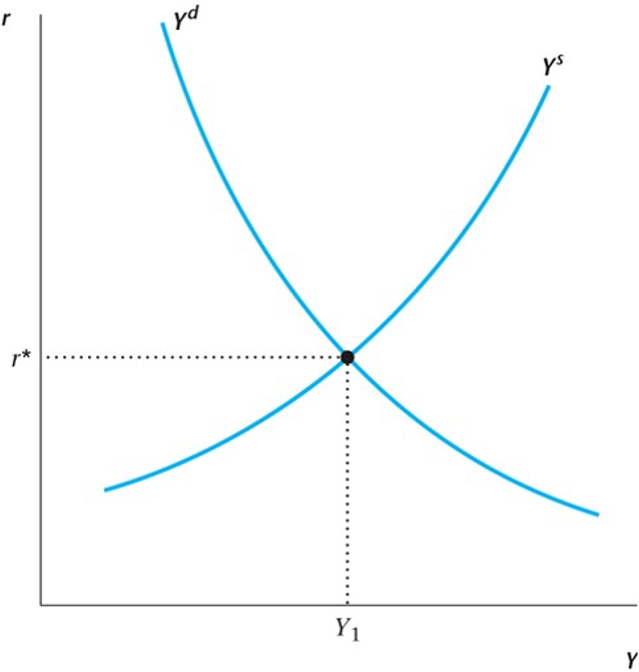
\includegraphics[scale=0.75]{Figures/W_Fig_17pt2.png}
\end{figure}
\end{frame}


\begin{frame}
\frametitle[alignment=center]{Exchange Rates Set by Money Supply \& Demand}
\begin{figure}
\centering
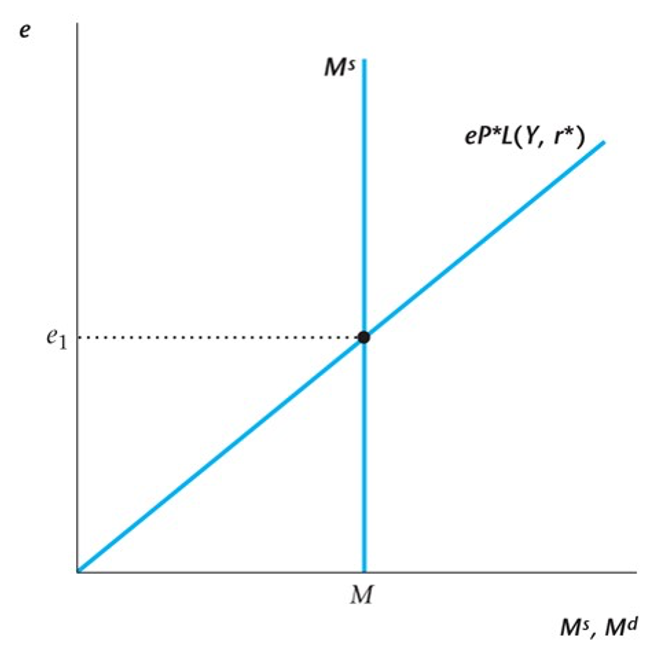
\includegraphics[scale=0.75]{Figures/W_Fig_17pt3.png}
\end{figure}
\end{frame}

\begin{frame}
\frametitle[alignment=center]{Experiment 1: Increase to $M$ with Flexible Exchange Rates}
\begin{itemize}
\item What happens if we increase the money supply 1\% from  $M_1$ to $M_s$?
\bigskip
\item As before, $P$ increases by 1\%
\bigskip
\item $e=\frac{P}{P^*}$, so the exchange rate increases by 1\%
\bigskip
\item Domestic currency ``depreciates" (can buy less of foreign currency) but real exchange rate is fixed
\bigskip
\item Could see it from:
$$\frac{M}{e}=P^*L(Y,r^*)$$
\item If $P^*$, $Y$, $r^*$ fixed, then $M/e$ is fixed
\bigskip
\item Note that right now we have flexible prices!  Sticky prices coming soon.
\end{itemize}
\end{frame}


\begin{frame}
\frametitle[alignment=center]{Exchange Rates Set by Money Supply \& Demand}
\begin{figure}
\centering
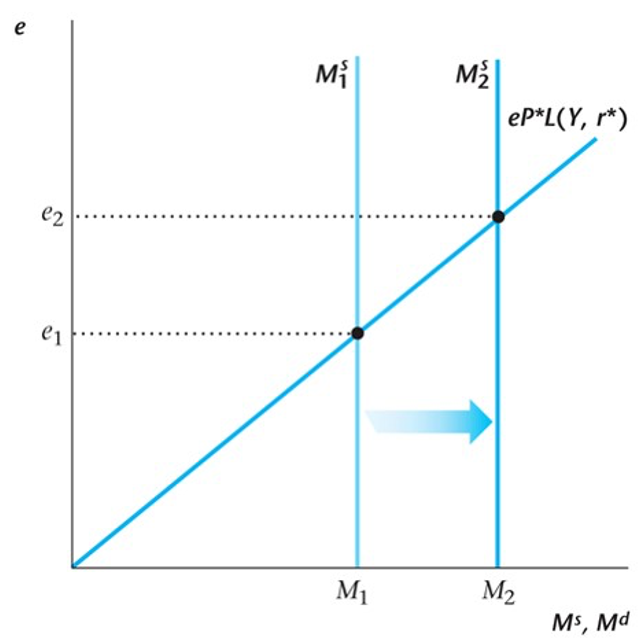
\includegraphics[scale=0.75]{Figures/W_Fig_17pt4.png}
\end{figure}
\end{frame}


\begin{frame}
\frametitle[alignment=center]{Experiment 2: Increase to $P^*$ with Flexible Exchange Rates}
\begin{itemize}
\item We saw what happens when $M$ increases
\bigskip
\item What if in the foreign country, $P^*$ increases (say because $M^*$ increased)
\bigskip
\item Then $eP^*$ increases (clockwise shift in money demand)
\bigskip
\item A fall in the exchange rate
\bigskip
\item $\frac{M}{P}=L(Y,r^*$ doesn't change, so $e=\frac{P^*}{P}$ determines $e$
\end{itemize}
\end{frame}


\begin{frame}
\frametitle[alignment=center]{Experiment 2: Increase to $P^*$ with Flexible Exchange Rates}
\begin{figure}
\centering
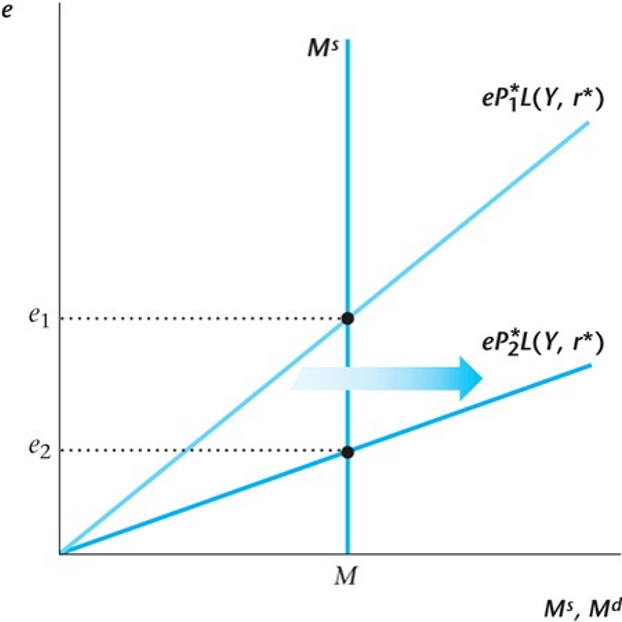
\includegraphics[scale=0.75]{Figures/W_Fig_17pt5.png}
\end{figure}
\end{frame}

\begin{frame}
\frametitle[alignment=center]{Experiment 3: Increase in world real interest rate}
\begin{itemize}
\item Now let's say global real interest rates increase from $r_1^*$ to $r_2^*$
\bigskip
\item $Y^d$ shifts out, $Y^s$ shifts out (not depicted) but total production rises
\bigskip
\item Increase in interest rates causes a decline in consumption and investment, though increase in income might rise consumption
\bigskip
\item As $r^*$ increases, output increases, so real money demand increases (assuming income effect > interest rate effect)
\bigskip
\item If money demand increases, while money supply stays same, then exchange rate should fall (dollar more valuable)
\end{itemize}
\end{frame}

\begin{frame}
\frametitle[alignment=center]{Experiment 3: Increase in world real interest rate}
\begin{figure}
\centering
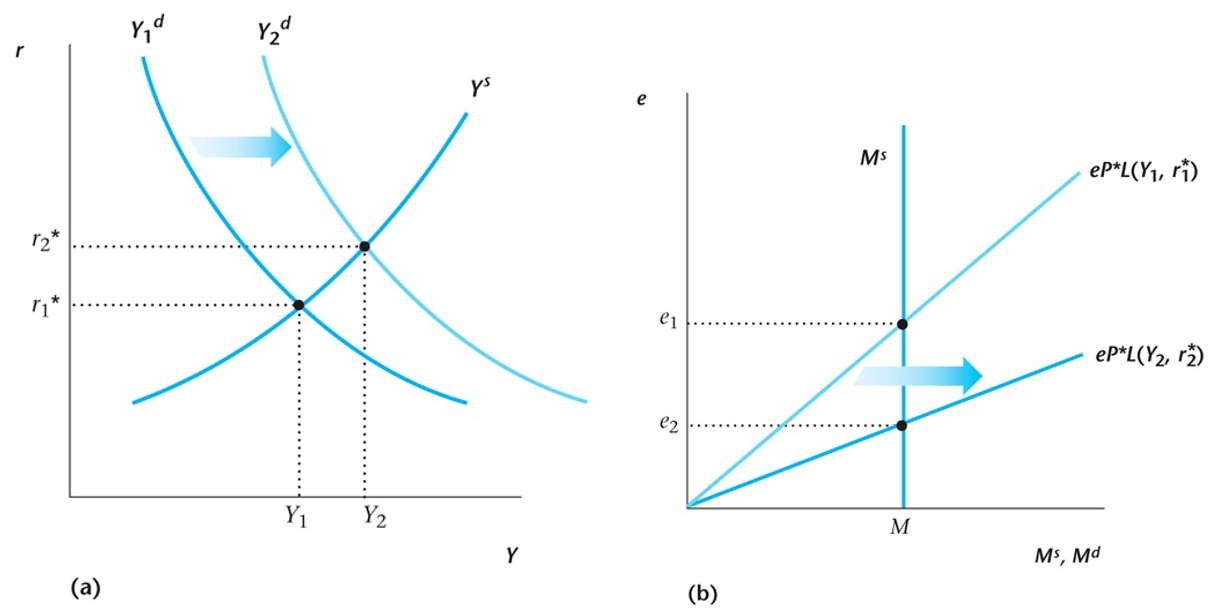
\includegraphics[scale=0.75]{Figures/W_Fig_17pt6.png}
\end{figure}
\end{frame}


\begin{frame}
\frametitle[alignment=center]{Pivoting to Fixed Exchange Rates}
\begin{itemize}
\item Now we pivot to fixed exchange rates
\bigskip
\item Difference is that now, central bank is going to fix $e$
\bigskip
\item Specifically, government says it will buy or sell foreign currency at a given price (must have foreign currency to do so!)
\begin{table}[ht!]
\centering
\begin{tabular}{lcc}
Assets & Liabilities \\
\hline
Foreign Exchange Reserves & Outside Money \\
 & Interest-Bearing Government Debt\\
 \hline
\end{tabular}
\end{table}
\item If desired exchange rate is 1 dollar for 1 pound, but market wants 1 dollar for 0.5 pounds (``too few" pounds, so they're more valuable), UK should sell pounds and buy dollars to depreciate (easy)
\item If desired exchange rate is 1 dollar for 1 pound, but market wants 1 dollar for 2 pounds (``too many" pounds, so they're not valuable enough) then UK should buy bounds and sell dollars to appreciate (hard!)
\end{itemize}
\end{frame}


\begin{frame}
\frametitle[alignment=center]{ Fixed Exchange Rates}
\begin{itemize}
\item Perhaps an easier way to see this is with money supply \& demand
\bigskip
\item To fix exchange rate, foreign country must adjust money supply 
\bigskip
\item Loses control of $M$ if it uses it to fix $e$
\bigskip
\item Now we can analyze:  rather than $P$ and $P^*$ determining $e$, fixed $e$ will determine $M$
\end{itemize}
\end{frame}


\begin{frame}
\frametitle[alignment=center]{ Experiment 1:  An Increase in the Foreign Price Level (fixed exchange rate)}
\begin{itemize}
\item Say that $P^*$ increases, and we're trying to fix our exchange rate to that country's currency
\bigskip
\item If $P=eP^*$, and $P^*$ increases, $e$ fixed, then it must be that $P$ increases
\bigskip
\item To increase $P$, we must increase $M$
\end{itemize}
\end{frame}



\begin{frame}
\frametitle[alignment=center]{Experiment 1:  An Increase in the Foreign Price Level (fixed exchange rate)}
\begin{figure}
\centering
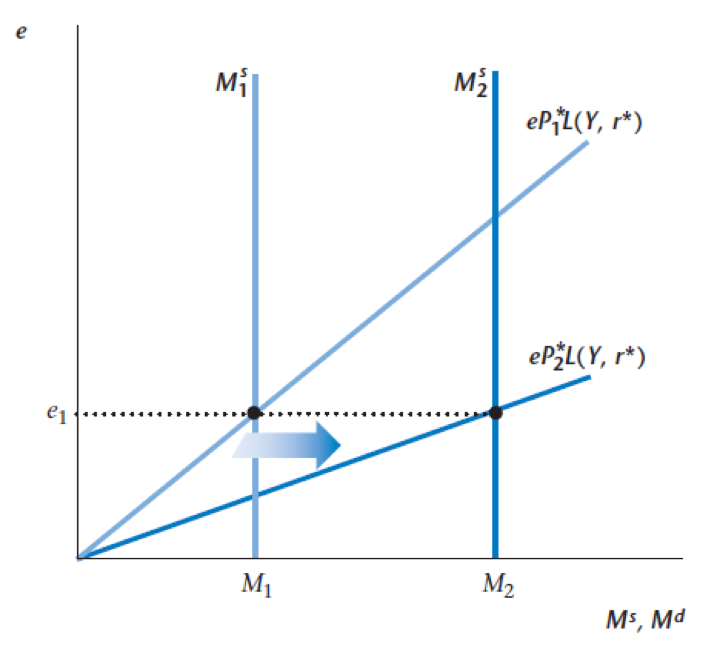
\includegraphics[scale=0.75]{Figures/W_Fig_17pt8.png}
\end{figure}
\end{frame}


\begin{frame}
\frametitle[alignment=center]{ Experiment 2:  A real foreign shock (fixed exchange rate)}
\begin{itemize}
\item Now let's say that $r_1^*$ increases to $r_2^*$
\bigskip
\item We again have an increase in domestic output, decrease in investment, ambiguous affect on consumption, and increase in CA
\bigskip
\item But recall that $eP^*L(Y_1,r_1^*)$ increases to $e(P')^*L(Y_2r_2^*)$
\bigskip
\item It must be that $M$ increases to offset increased domestic demand for currency
\end{itemize}
\end{frame}


\begin{frame}
\frametitle[alignment=center]{Experiment 2:  A real foreign shock (fixed exchange rate)}
\begin{figure}
\centering
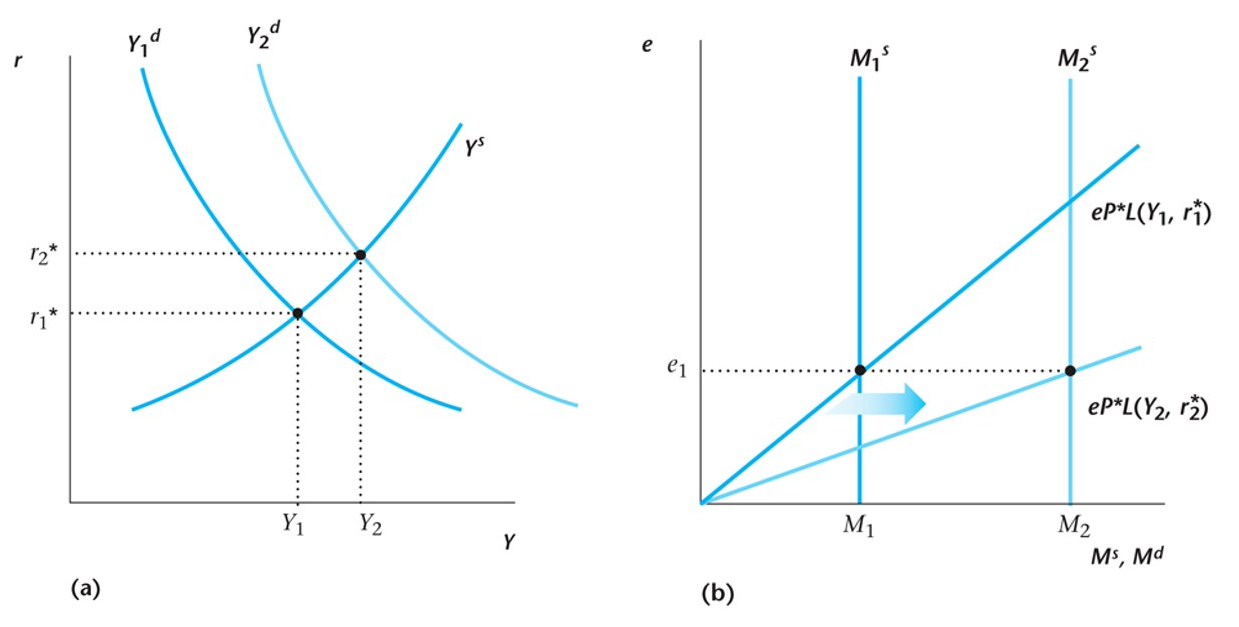
\includegraphics[scale=0.75]{Figures/W_Fig_17pt9.png}
\end{figure}
\end{frame}



\begin{frame}
\frametitle[alignment=center]{ Experiment 3:  Devaluation}
\begin{itemize}
\item What happens if the economy is hit with a negative productivity shock?
\bigskip
\item Normally, the exchange rate would rise (local prices rise)
\bigskip
\item To fight inflation/exchange rate appreciating, government would have to shift in money supply
\bigskip
\item But this is expensive!  Government has to buy back money.
\bigskip
\item So tension between desire to keep $e$ and desire to not lose money via $M_1\rightarrow M_2$, $M_2<M_1$.
\end{itemize}
\end{frame}

\begin{frame}
\frametitle[alignment=center]{Experiment 3:  TFP shock--devaluation, or defend?}
\begin{figure}
\centering
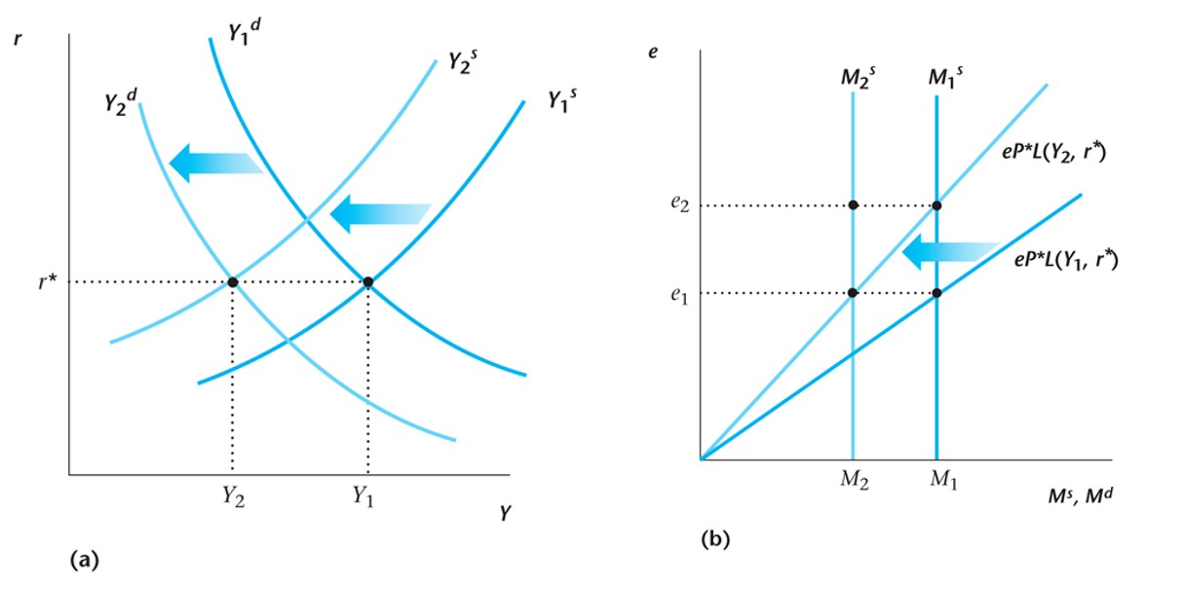
\includegraphics[scale=0.7]{Figures/W_Fig_17pt10.png}
\end{figure}
\end{frame}


\begin{frame}
\frametitle[alignment=center]{ Flexible vs. Fixed Exchange Rates}
\begin{itemize}
\item What's better, a flexible or a fixed exchange rate?
\bigskip
\item Flexible exchange rate helps absorb nominal shock in a foreign price level, stabilizes domestic prices
\bigskip
\item But fixed exchange rate means real shocks from abroad have a small effect on local price level, by acting as shock absorber
\bigskip
\item Flexible exchange rate means you have control over your own monetary policy--could be good or bad!
\end{itemize}
\end{frame}

\begin{frame}
\frametitle[alignment=center]{ Balance of Payments}
\begin{itemize}
\item We need to understand the capital account \& balance of payments, so we can talk about capital controls
\bigskip
\item When foreigners buy a U.S. asset, it is a positive capital inflow, when a U.S. citizen buys a foreign asset, it is a capital outflow
\bigskip
\item If funds flow into your country to buy assets, it's an inflow.
\bigskip
\item Balance of payments is current account surplus plus capital account surplus:
$$BP=KA+CA$$
\item Balance of payments should always be zero:
$$KA=-CA$$
\item Idea is that if a country is sending you things on net (I get an iPhone, but send them no good or service back), then it must be that I owe them something (they have an asset in this country, possibly debt, or cash).  
\end{itemize}
\end{frame}

\begin{frame}
\frametitle[alignment=center]{ Capital Controls}
\begin{itemize}
\item Now, it might make sense how capital controls affect trade!
\bigskip
\item $KA=-CA$
\bigskip
\item Say we're hit with a decrease in TFP, so $Y^s$ falls
\bigskip
\item If $r$ is fixed, then total demand falls until equilibrium $r$ is the global $r$, total income falls
\bigskip
\item But if trade is banned, and $r$ is flexible, then $Y^d$ doesn't fall, so total $Y$ doesn't fall by as much
\bigskip
\item Another way of thinking about it:  if our economy less productive, if we can trade we can smooth consumption by importing rather than making things inefficiently at home, going into debt.  If we're banned from trading, economy ``sucks it up" and works more than if it had debt available.
\end{itemize}
\end{frame}

\begin{frame}
\frametitle[alignment=center]{Capital Controls (Flexible $e$)}
\begin{figure}
\centering
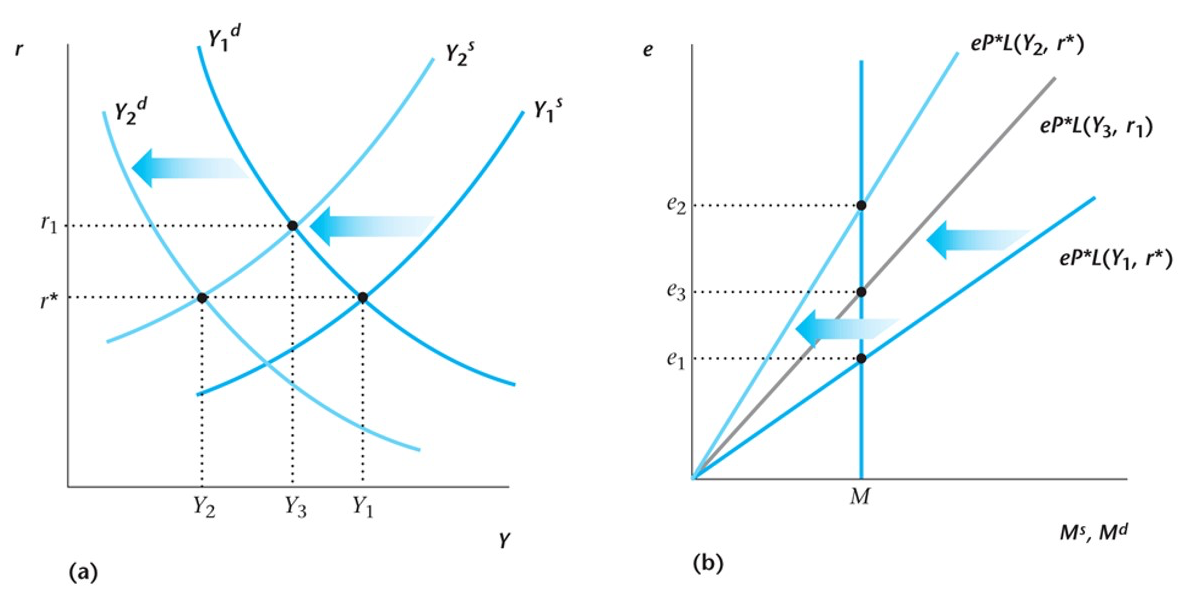
\includegraphics[scale=0.7]{Figures/W_Fig_17pt11.png}
\end{figure}
\end{frame}

\begin{frame}
\frametitle[alignment=center]{Capital Controls (Fixed $e$)}
\begin{figure}
\centering
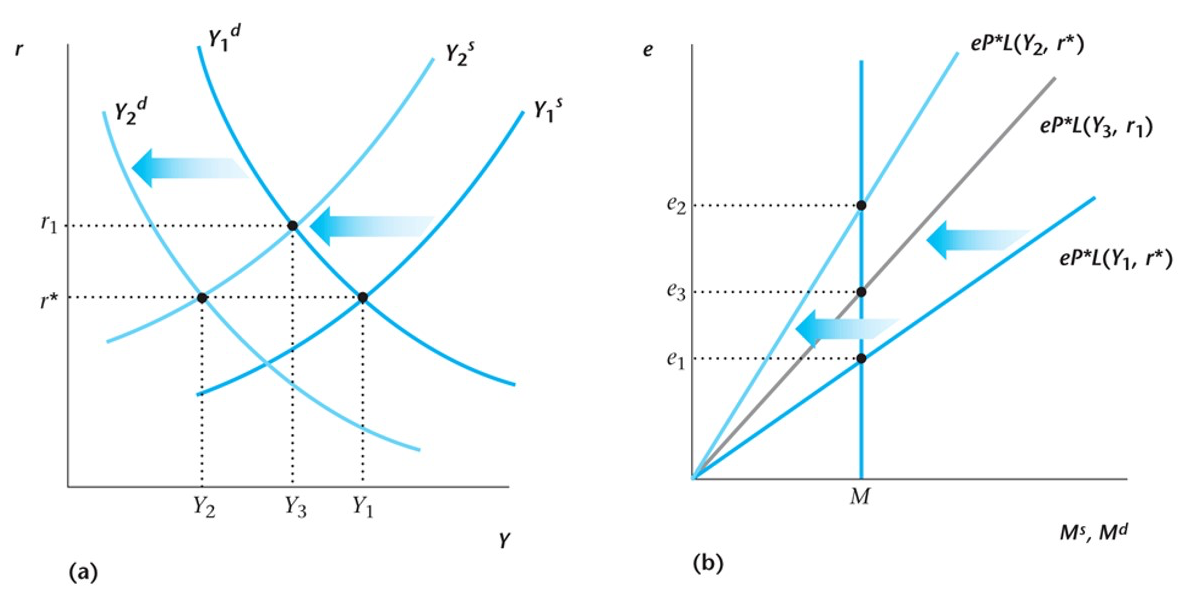
\includegraphics[scale=0.7]{Figures/W_Fig_17pt11.png}
\end{figure}
\end{frame}


\begin{frame}
\frametitle[alignment=center]{Capital Controls in Practice}
\begin{itemize}
\item Controlling capital is hard
\bigskip
\item  Example from Chile:  any time you purchased Chilean assets, you had to hold some of it at the Bank of Chile, at no interest
\bigskip
\item But investors just avoided the controls (many clever schemes)
\end{itemize}
\end{frame}



\begin{frame}
\frametitle[alignment=center]{Net Export Demand}
\begin{itemize}
\item Now we want to combine our New Keynesian model with our trade model
\bigskip
\item Some goods made domestically, some internationally, but both are \emph{imperfect substitutes} for one another
\bigskip
\item Net exports is a positive function of the real exchange rate: $NX\left(\frac{eP^*}{P}\right)$
\begin{itemize}
\item When takes more dollars buy less foreign currency ($e\uparrow$), export more/import less
\bigskip
\item When foreign prices are higher  ($P^*\uparrow$), export more/import less
\bigskip
\item When local prices are higher ($P\uparrow$), export less/import more
\end{itemize}
\item Real exchange rate:  when I give up fewer local goods to buy foreign goods, I do so
\end{itemize}
\end{frame}

\begin{frame}
\frametitle[alignment=center]{A New Keynesian Sticky Price Open-Economy Model}
\begin{itemize}
\item Now, $P_1$ is fixed, $r^*$ is fixed (globally) and $M^s$ is fixed
\bigskip
\item Money market determines $Y$ $M^s=PL(Y,r)$, but $M^s$, $P$, and $r$ are set, so $Y$ moves to clear money supply=money demand
\end{itemize}
\end{frame}

\begin{frame}
\frametitle[alignment=center]{New Keynesian Model with Flexible Exchange Rate}
\begin{figure}
\centering
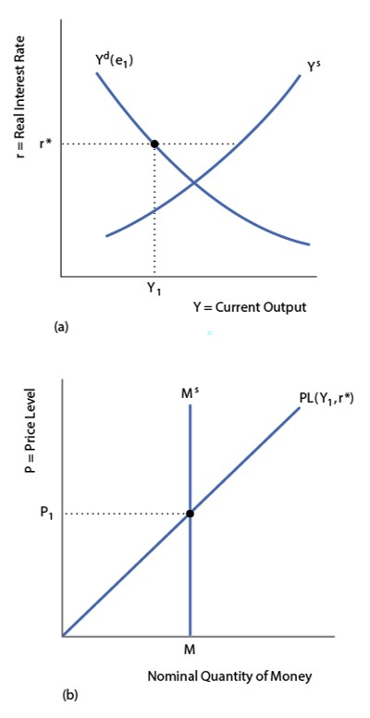
\includegraphics[scale=0.55]{Figures/W_Fig_17pt13.png}
\end{figure}
$Y$ is pinned down by $M^s$ (exogenous), $P$ (fixed) and $r$ (global)
\end{frame}

\begin{frame}
\frametitle[alignment=center]{Monetary Policy}
\begin{itemize}
\item Now, if $P$, $r$, $M$ are fixed, when $M^s$ shifts out, $P$ can't rise, and central bank doesn't control $r$!
\bigskip
\item Because $P$ is fixed in the short run, $P=eP^*$ doesn't hold (purchasing power parity doesn't hold in short run)
\bigskip
\item When $M^s$ increases, $e$ rises (dollars more plentiful, so more dollars to buy one unit of foreign currency), increasing net export demand
\bigskip
\item In other words, home goods are cheaper to foreigners now, so they demand more
\bigskip
\item Output demand shifts out, and GDP rises
\bigskip
\item This worked similarly to the closed Keynesian model, but now it went $M\uparrow\rightarrow e\uparrow \rightarrow NX\uparrow\rightarrow Y^d\uparrow$
\end{itemize}
\end{frame}


\begin{frame}
\frametitle[alignment=center]{Monetary Policy (Flexible Exchange Rate)}
\begin{figure}
\centering
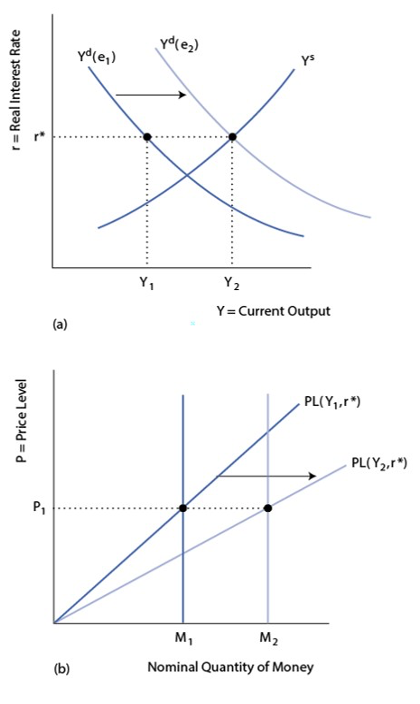
\includegraphics[scale=0.55]{Figures/W_Fig_17pt14.png}
\end{figure}
As $M$ shifts out, $e$ rises, $NX\left(\frac{eP^*}{P}\right)$ rises, so $Y^d$ rises
\end{frame}

\begin{frame}
\frametitle[alignment=center]{Fiscal Policy}
\begin{itemize}
\item Now let's say $G$ increases
\bigskip
\item $M=PL(Y,r)$ determines $Y$, and if $M$ $P$, $r$ fixed, then $Y$ is too.
\bigskip
\item If $Y$ is fixed, but govt now demanding more, it must be that $NX$ falls ($e$ falls)
\bigskip
\item Nothing changes, government spending crowds out exports
\end{itemize}
\end{frame}

\begin{frame}
\frametitle[alignment=center]{Monetary Policy (Flexible Exchange Rate)}
\begin{figure}
\centering
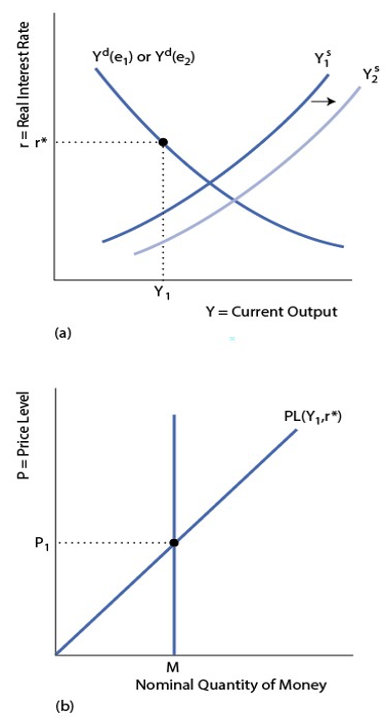
\includegraphics[scale=0.55]{Figures/W_Fig_17pt15.png}
\end{figure}
As $G$ shifts out, $e$ shifts down (more demand for dollars), $NX\left(\frac{eP^*}{P}\right)$ falls, and $Y$ stays same
\end{frame}




\begin{frame}
\frametitle[alignment=center]{Fixed Exchange Rates}
\begin{itemize}
\item Again, consider an increase in $G$, but under fixed exchange rates (monetary policy passive, fixing $e$)
\bigskip
\item Now, as $G$ increases, $e$ would fall (more demand for dollars!), but to counteract, Fed increases money supply.  Real incomes fall, and $Y^s$ and $Y^d$ both rise, just as before, equilibrating at $r^*$ (if $G$ chosen correctly)
\end{itemize}
\end{frame}


\begin{frame}
\frametitle[alignment=center]{Fiscal  Policy (Fixed Exchange Rate)}
\begin{figure}
\centering
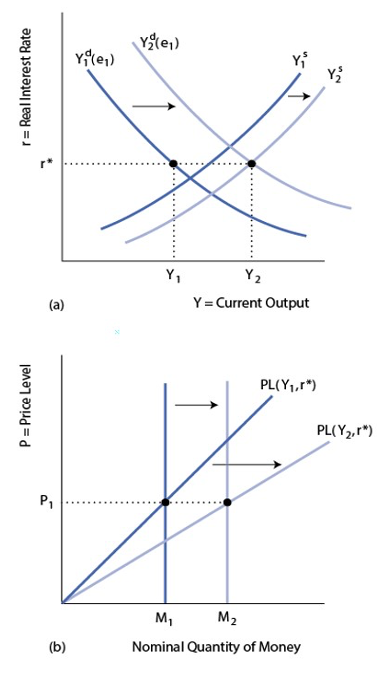
\includegraphics[scale=0.55]{Figures/W_Fig_17pt16.png}
\end{figure}
As $G$ shifts out, $e$ shifts down (more demand for dollars), $NX\left(\frac{eP^*}{P}\right)$ falls, and $Y$ stays same
\end{frame}


\begin{frame}
\frametitle[alignment=center]{Conclusions}
\begin{itemize}
\item Famous model in Macro, the ``Mundell-Fleming" model widely taught
\bigskip
\item But has embarssing assumptions (downward-sloping ``IS" curve) 
\bigskip
\item This NK model recovers one of the big findings:
\begin{itemize}
\item When you have fixed exchange rate, monetary policy is not effective (must move to fix exchange rate)
\bigskip
\item When you have a flexible exchange rate, fiscal policy is not effective (increased demand for dollars decreases $e$ and thus $NX$, offsetting increase)
\end{itemize}
\bigskip
\item Now you have a model of exchange rates!
\end{itemize}
\end{frame}



\end{document}